\chapter{\kadaie}
\section{\purpose}
脳波は以下のように説明されている.
\begin{quote}
    ``神経細胞の間にあるシナプス電位と,後電位などの電極変動の総和を,頭皮上に付けた電極を用いて記録したもの.''
    \\\hfill\cite{自己心理学セミナー}
\end{quote}
また,特定の事象に関係する脳波を「事象関連電位(ERP)」と呼ぶ.脳波測定で,ERPを電極で測定する.
BMI(Brain Machine Interfae)とは,脳からの信号を計測し,それを利用する技術を指す\cite{脳波による実用的なBMI研究開発}.
これまで,BMIを用いた家電の操作や,文字入力操作が研究されている\cite{脳波による実用的なBMI研究開発}.
\paragraph{目的}BMIのシステムを体験するために,タイプしたい文字を脳情報から読み取る.具体的に,ターゲット刺激が表示されたときの脳波と,ターゲット刺激でない刺激が表示されたときの脳波を比較する.
\section{\method}
\paragraph{実験装置}
刺激呈示用装置として,汎用コンピュータと液晶ディスプレイを利用する.
脳波計測機器やコンピュータなどの実験装置を\tblref{tbl:実験装置\kadaie}に示す.実験参加者は,学生の20代男性1名である.
\begin{table}[H]
    \caption{実験装置\ (\kadaie)}
    \label{tbl:実験装置\kadaie}
    \begin{tabularx}{\textwidth}{cAR}
        \hline
        \multirow{3}{*}{\bfseries BMI装置}  & 電極       & ドライ電極                                            \\
                                          & 脳波計測機器   & \texttt{g.USBamp}                                \\
                                          & 分析ソフトウェア & \texttt{g.BSanalyze}                             \\
        \hline
        \multirow{6}{*}{\bfseries コンピュータ} & コンピュータ   & Dell Precision M6600 64-bit Operating System     \\
                                          & プロセッサ    & Intel(R) Core(TM) i7-2620M SPC @ 2.70GHz 2.70GHz \\
                                          & メモリ      & 8GB (7.88GB usable)                              \\
                                          & OS       & Windows 7 Ultimate Service Pack 1                \\
                                          & \matlab  & バージョン不明                                          \\
                                          & Simulink & バージョン不明                                          \\
        \hline
    \end{tabularx}
\end{table}
\textbf{用語解説}
\begin{itemize}
    \item \textbf{p300}:
          p300とは,刺激呈示後,潜時約\(300\textrm{ms}\)に出現する陽性成分のことを指す\cite{P300基礎}.
    \item \textbf{参照電極}:
          基準電極とも呼ばれる.測定する電位の基準値を測定するための電極である.神経細胞がなく,電位が一定である耳たぶを採用している.
    \item \textbf{接地電極}:
          計測した電位を再び戻すために利用する.これにより,データを計測しやすくする.位置は額.
\end{itemize}
\textbf{実験の手続き}
\begin{multicols}{2}
    \begin{enumerate}
        \item \matlab からSimulinkのブロックセットを起動し,ドライ電極を頭部に装着する\footnotemark[1].
        \item 電極(\texttt{Fz},\texttt{Cz},\texttt{Pz},\texttt{P4},\texttt{PO7},\texttt{Oz},\texttt{PO8})を\figref{fig:電極の配置図}に従ってセットする.参照電極は耳たぶに,接地電極を額にセットする.対象が視覚刺激のため,後頭部に電極が集中している.
        \item 実験参加者は,PC上に表示された\(6\times6\)行列の文字を観察する.灰色の英字または数字が黒の背景上に呈示され,その中からランダムな順で\(1\)文字が\(100\textrm{ms}\)だけ白に変わる.その後,\(75\textrm{ms}\)はどの文字も灰色となり,その後また別の文字が白くなる.
        \item 実験参加者は集中して画面を注視し,指定された文字が白く変わるたびにその回数を数える.今回は\texttt{KUT}の3文字とする.
              \columnbreak
        \item トレーニングモードでは各文字が各行列で10回ずつ表示される.
        \item トレーニングモードのデータ測定が終了したら,\texttt{g.BSanalyze}を起動し,トレーニングデータを読み込む.\texttt{KUT}が白く表示されたとき(target条件)とそうでないとき(non-target条件)の波形規則を学習させ,判定機を作成する.今回は線形判別分析(LDA)を用いる.
        \item target条件とnon-target条件をそれぞれ加算平均したグラフを出力する.
        \item \text{フラッシュ}回数は5回として,テストモードで同様のタイピング実験をする.
    \end{enumerate}
\end{multicols}
\begin{figure}[H]
    \centering
    \begin{minipage}[b]{.32\textwidth}
        \centering
        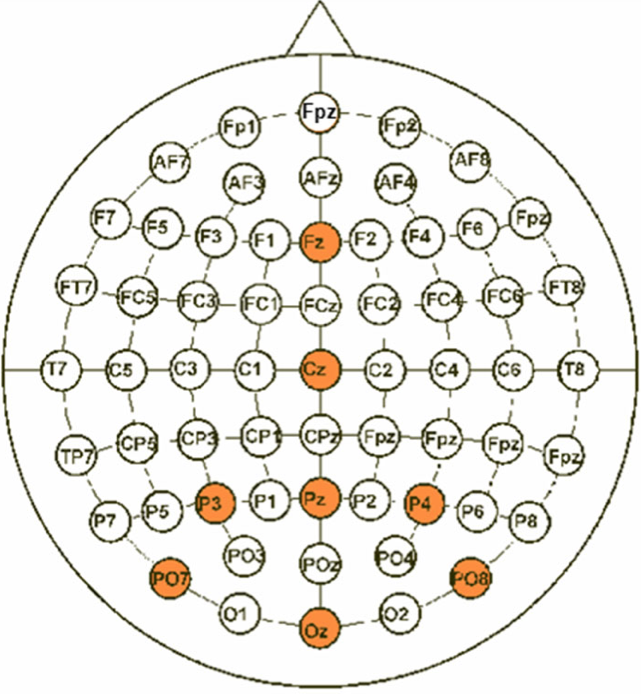
\includegraphics[keepaspectratio,width=.6\textwidth]{../../12_DataAnalysis/denkyoku.png}
        \caption{電極の配置図\footnotemark[2]}
        \label{fig:電極の配置図}
    \end{minipage}
    \begin{minipage}[b]{.32\textwidth}
        \centering
        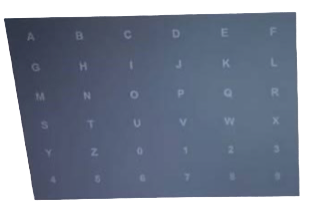
\includegraphics[keepaspectratio,width=.6\textwidth]{../../12_DataAnalysis/bmi-shigeki.png}
        \caption{呈示される刺激(例)}
    \end{minipage}
    \begin{minipage}[b]{.32\textwidth}
        \centering
        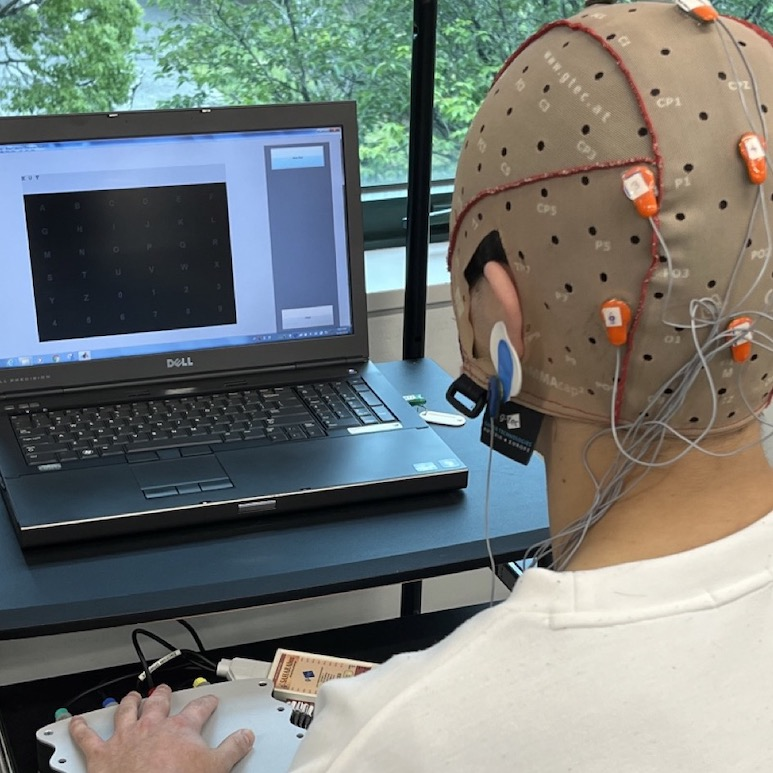
\includegraphics[keepaspectratio,width=.6\textwidth]{../../12_DataAnalysis/bmi_exp2.jpeg}
        \caption{テストモードの実験}
    \end{minipage}
\end{figure}
\footnotetext[1]{サンプリング周波数\(256\textrm{Hz}\),データに対して\(0,1〜30\textrm{Hz}\)のバンドパスフィルタを通し,低周波の大きな電位変化と高周波のノイズを除去する.}
\footnotetext[2]{KUT-LMS 課題説明資料(\url{https://lms.kochi-tech.ac.jp/pluginfile.php/209127/mod_resource/content/12/task0529.pdf})より}
\section{\result}
実験結果を\figref{fig:実験結果\kadaie}に示す.凡例の電極と2つのグラフは1対1で対応している.
\begin{figure}[H]
    \centering
    \begin{minipage}[b]{.3\textwidth}
        \centering
        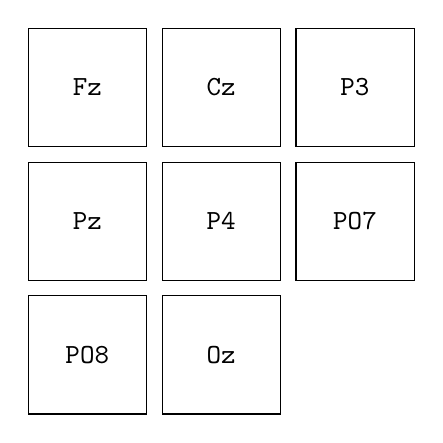
\begin{tikzpicture}
            \draw(0,0)rectangle (1.5,1.5)node[midway]{\texttt{PO8}};
            \draw(1.7,0)rectangle (3.2,1.5)node[midway]{\texttt{Oz}};

            \draw(0,1.7)rectangle (1.5,3.2)node[midway]{\texttt{Pz}};
            \draw(1.7,1.7)rectangle (3.2,3.2)node[midway]{\texttt{P4}};
            \draw(3.4,1.7)rectangle (4.9,3.2)node[midway]{\texttt{PO7}};

            \draw(0,3.4)rectangle (1.5,4.9)node[midway]{\texttt{Fz}};
            \draw(1.7,3.4)rectangle (3.2,4.9)node[midway]{\texttt{Cz}};
            \draw(3.4,3.4)rectangle (4.9,4.9)node[midway]{\texttt{P3}};
        \end{tikzpicture}
        \subcaption{凡例}
    \end{minipage}
    \begin{minipage}[b]{.3\textwidth}
        \centering
        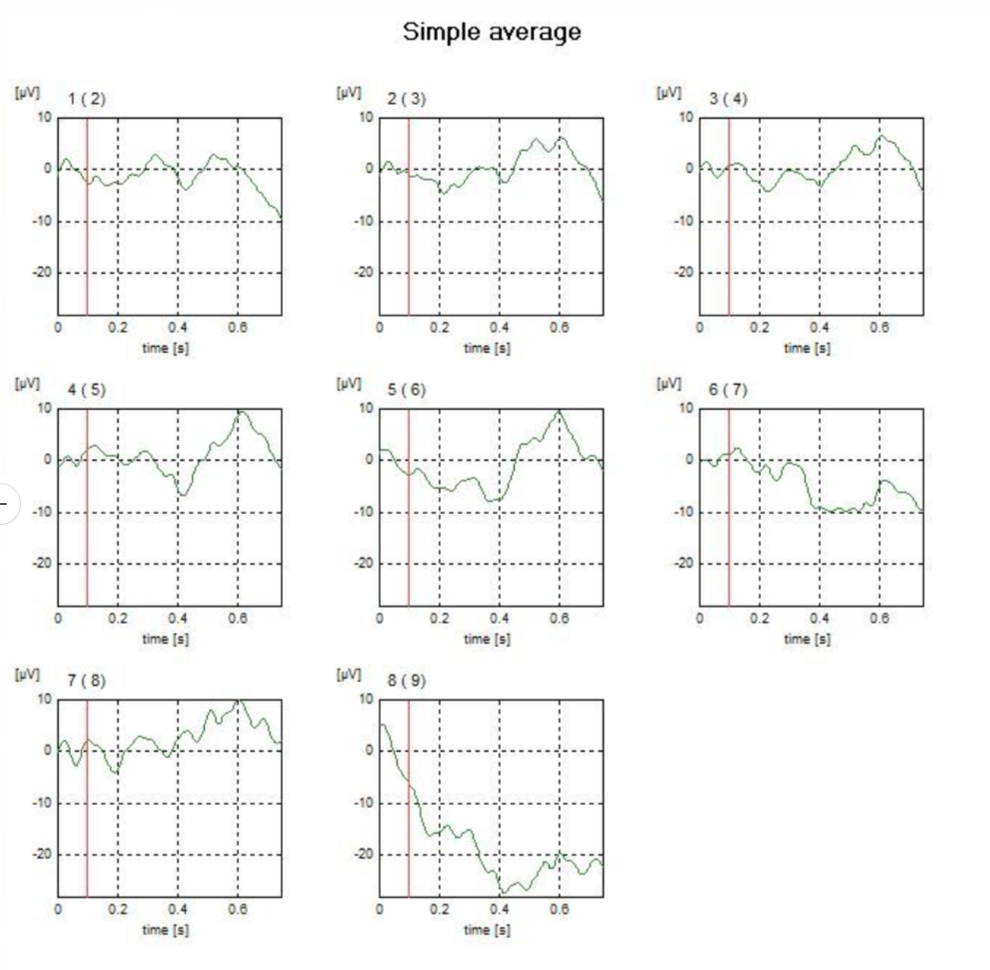
\includegraphics[keepaspectratio,width=\textwidth]{../../12_DataAnalysis/bmi_target.png}
        \subcaption{target条件}
    \end{minipage}
    \begin{minipage}[b]{.3\textwidth}
        \centering
        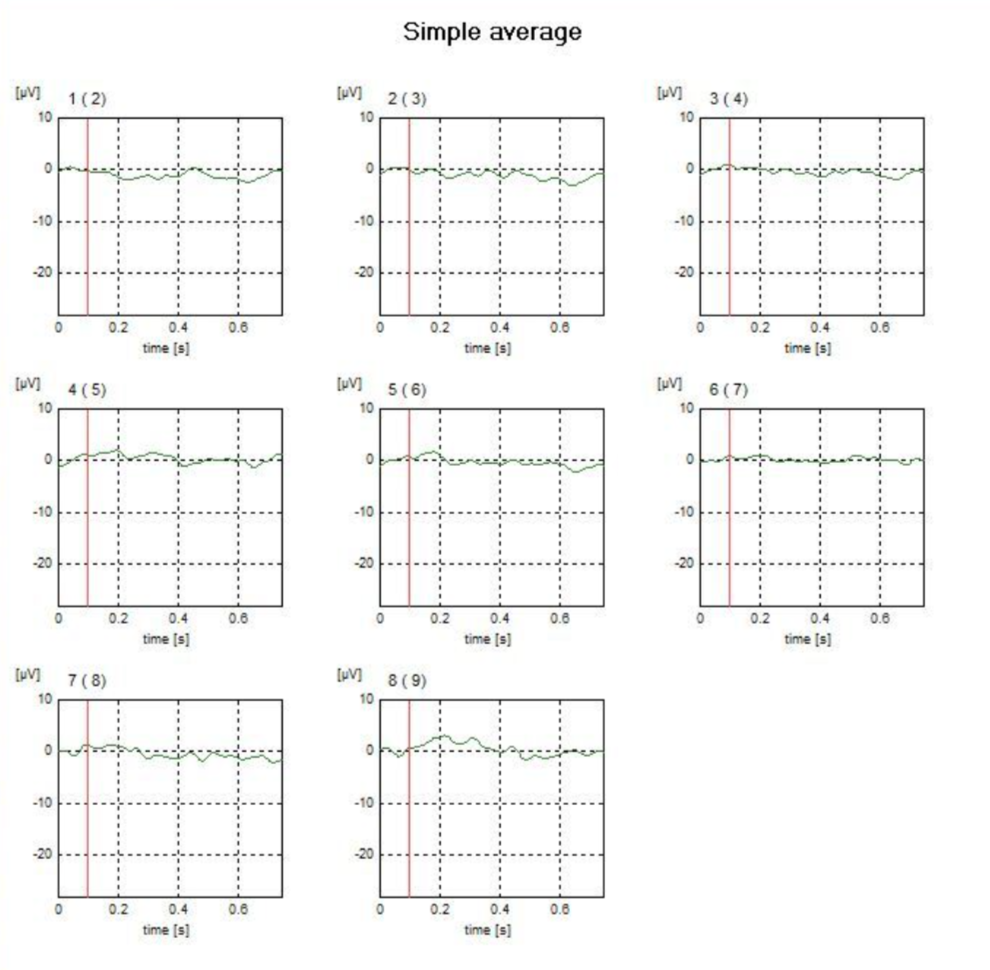
\includegraphics[keepaspectratio,width=\textwidth]{../../12_DataAnalysis/bmi_nontarget.png}
        \subcaption{non-target条件}
    \end{minipage}
    \caption{\kadaie 実験結果}
    \label{fig:実験結果\kadaie}
\end{figure}
\clearpage
\section{\consideration}
結果(\figref{fig:実験結果\kadaie})を比較すると,target条件の方がnon-target条件に比べて電位の振れが大きい.
これは,刺激に反応していると考えられる.しかし,特に\texttt{Oz}電極では電位が負に振れており,この原因は分からなかった.
\section{\conclusion}
本実験により,target条件下とnon-target条件下では脳波に大きな違いが出た.
しかしp300は刺激呈示後,陽性成分をさしており,通常であれば電位が正向きに振れる.結果の一部は大きく負に振れており,この原因は分からなかった.